\chapter{Sprint 1 : Fondation, Accès et Profils} 
\minitoc
\newpage

\section{Introduction}
Ce troisième chapitre marque le début de la phase de réalisation pratique de notre projet. Conformément à la méthodologie Agile Scrum adoptée, le premier sprint est fondamental car il vise à mettre en place l'architecture socle de l'application "CoachingApp". Durant cette itération de trois semaines, nous nous sommes concentrés sur la modélisation et l'initialisation de la base de données relationnelle, le déploiement du serveur Node.js, et la mise en œuvre des mécanismes de sécurité cruciaux, notamment l'authentification et l'autorisation. Enfin, nous avons développé les premières interfaces mobiles en Flutter pour permettre la création de comptes, la complétion des profils biométriques, et la gestion des demandes de mise en relation entre les athlètes et les coachs.

\section{Objectifs et Planification du Sprint}
Le Sprint Planning a permis à l'équipe de sélectionner un ensemble cohérent de User Stories depuis le Product Backlog, afin de livrer un incrément fonctionnel.

\subsection{Backlog du Sprint 1}
Les objectifs spécifiques convertis en tâches de développement sont les suivants :
\begin{itemize}
    \item \textbf{Tâche Backend 1.1 :} Configurer le projet Node.js avec TypeScript, Express et TypeORM.
    \item \textbf{Tâche Backend 1.2 :} Modéliser les entités \texttt{User}, \texttt{Athlete}, et \texttt{CoachProfile} dans PostgreSQL.
    \item \textbf{Tâche Backend 1.3 :} Implémenter l'algorithme de hachage bcrypt et la génération de tokens JWT pour la route \texttt{POST /api/auth/login}.
    \item \textbf{Tâche Frontend 1.1 :} Initialiser le projet Flutter et mettre en place l'architecture BLoC (Business Logic Component) ou Provider pour la gestion d'état.
    \item \textbf{Tâche Frontend 1.2 :} Développer les écrans \textit{LoginScreen} et \textit{RegisterScreen} avec validation des formulaires.
    \item \textbf{Tâche Fullstack 1.1 :} Mettre en place le système de "Coaching Requests" (Création de la route API, intégration UI de la recherche de coach).
\end{itemize}

\section{Conception détaillée du Sprint 1}
Avant d'écrire la moindre ligne de code, les fonctionnalités de ce sprint ont été rigoureusement modélisées.

\subsection{Diagramme de cas d'utilisation (Sprint 1)}
Le diagramme de cas d'utilisation du Sprint 1 illustre les interactions des acteurs pour la création de compte, l'authentification et la gestion des profils. Il met en évidence la séparation des rôles une fois l'utilisateur connecté.

\begin{figure}[H]
\centering
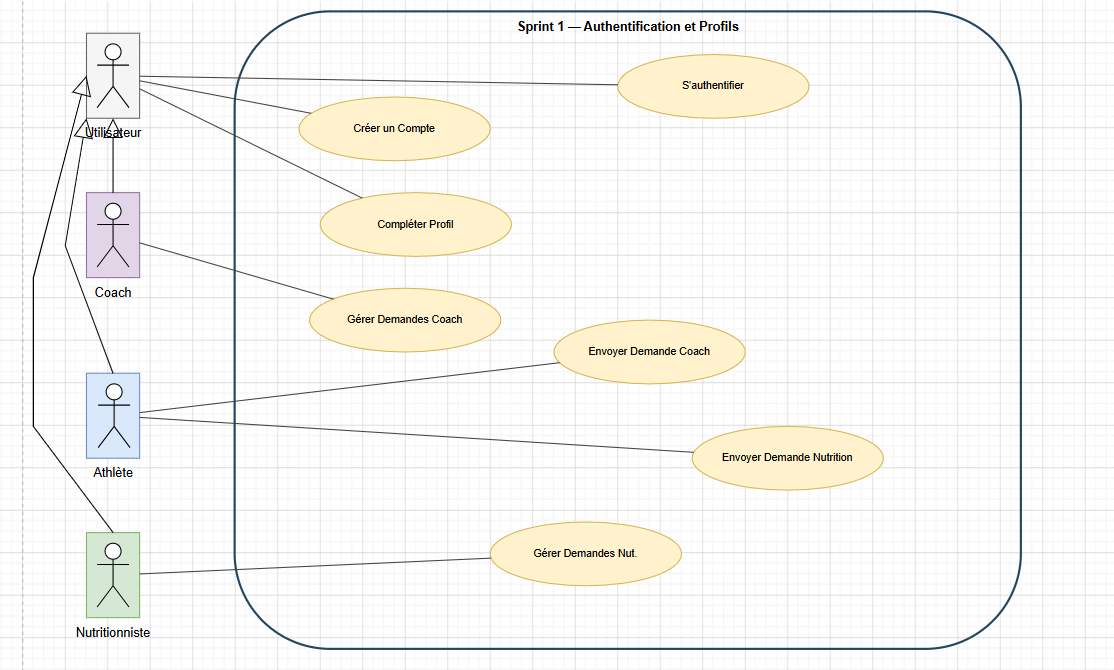
\includegraphics[width=0.85\textwidth]{diagrams/use case sprint 1.png}
\caption{Diagramme des cas d'utilisation - Sprint 1}
\end{figure}

\subsection{Diagramme de classes (Sprint 1)}
Ce diagramme détaille les entités nécessaires pour la gestion des utilisateurs, des profils spécifiques et des demandes de coaching. Le choix d'une relation "Un-à-Un" (One-to-One) entre \texttt{User} et \texttt{Athlete} (ou \texttt{CoachProfile}) permet de garder une table d'authentification légère tout en isolant les données métiers spécifiques.

\begin{figure}[H]
\centering
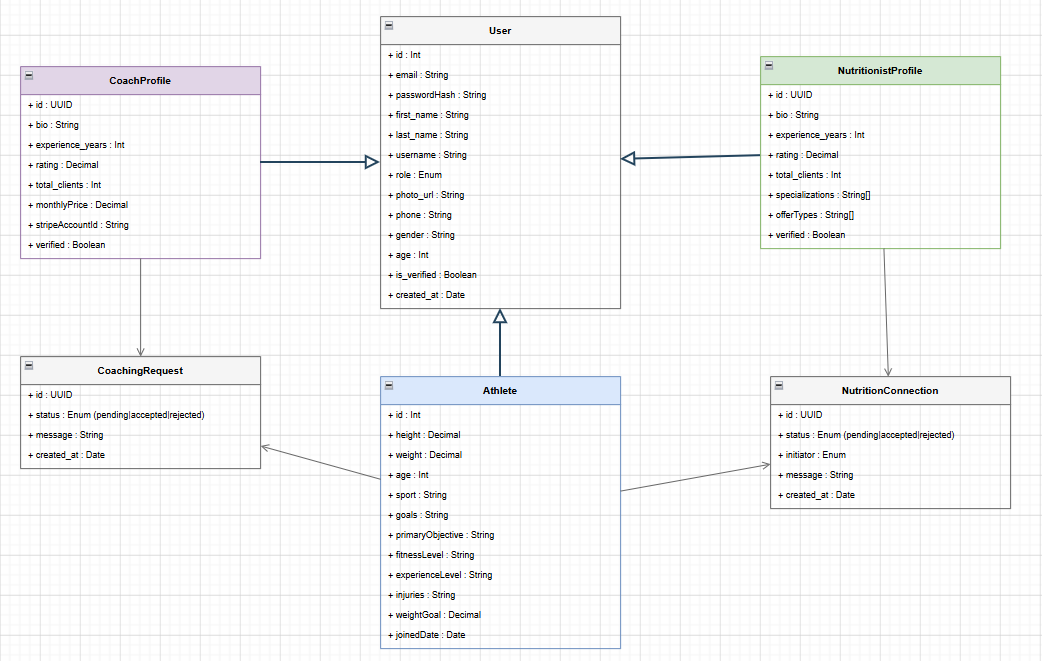
\includegraphics[width=1\textwidth]{diagrams/classe sprint 1.png}
\caption{Diagramme de classes - Sprint 1}
\end{figure}

\subsection{Diagramme de séquence : S'authentifier}
Le processus d'authentification est une étape critique de l'application. La sécurité doit être infaillible pour protéger les données de santé. Le diagramme de séquence suivant illustre le flux complet : l'utilisateur fournit ses informations d'identification au client Flutter, qui les transmet via une requête HTTP POST sécurisée à l'API Node.js. L'API interroge PostgreSQL. En cas de succès (mot de passe valide après vérification bcrypt), le serveur génère un JSON Web Token (JWT) signé avec une clé secrète, qui est renvoyé au client.

%[Note : Ajoutez l'image exportée depuis PlantUML dans le dossier diagrams/ avec ce nom]
\begin{figure}[H]
\centering
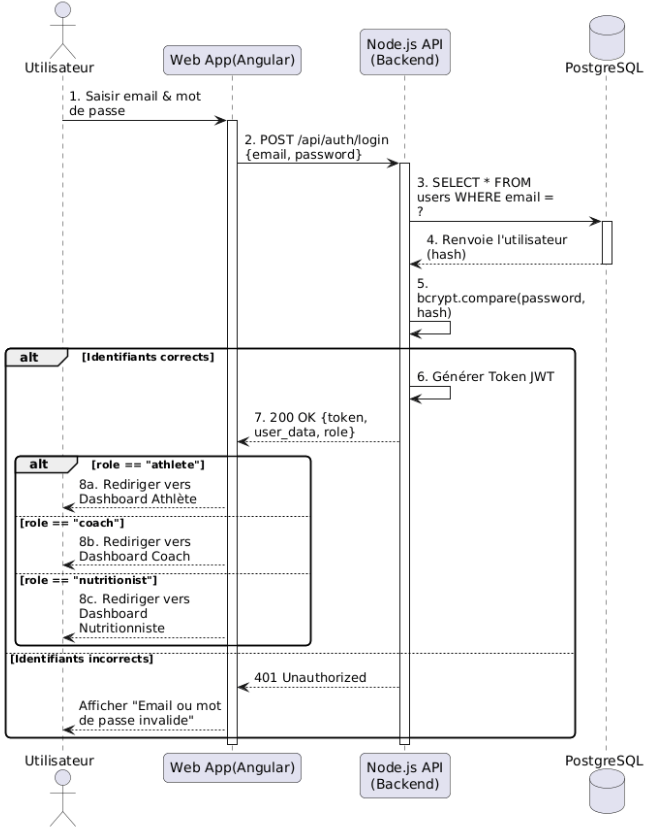
\includegraphics[width=0.85\textwidth]{diagrams/sequence sprint 1.png}
\caption{Diagramme de séquence : S'authentifier}
\end{figure}

\section{Réalisation technique et Implémentation}

\subsection{Environnement de développement et Outils}
Pour garantir la qualité et la vélocité du développement lors de ce sprint, nous avons configuré les environnements suivants :
\begin{itemize}
    \item \textbf{VS Code (Visual Studio Code) :} Éditeur de code principal, enrichi d'extensions pour l'analyse statique du code (ESLint pour TypeScript, Dart Analyze pour Flutter).
    \item \textbf{Postman :} Outil indispensable pour tester et valider isolément les différents endpoints de notre API REST (ex: tester les erreurs 401 Unauthorized, 400 Bad Request) avant même que l'interface mobile ne soit développée.
    \item \textbf{PgAdmin 4 / DBeaver :} Interfaces graphiques avancées pour l'administration et la visualisation des schémas de notre base de données PostgreSQL locale.
    \item \textbf{Git \& GitHub :} Gestionnaire de versions utilisé pour maintenir l'historique du code et résoudre les conflits lors de fusions de branches.
\end{itemize}

\subsection{Implémentation du Backend (Node.js / TypeORM)}
La première étape fut la création des modèles de données. Grâce à TypeORM, nous avons mappé nos objets TypeScript en tables SQL.

\subsubsection{Héritage et Modélisation des Utilisateurs}
Dans CoachingApp, un utilisateur peut être un Coach, un Athlète ou un Nutritionniste. Plutôt que de créer une table monolithique géante remplie de valeurs nulles, nous avons utilisé des tables de profils liées par des clés étrangères, ce qui normalise la base de données (3ème forme normale).

\begin{lstlisting}[language=JavaScript, caption={Extrait de l'entité User sous TypeORM}, label={lst:user_entity}]
@Entity('users')
export class User {
  @PrimaryGeneratedColumn('uuid')
  id: string;

  @Column({ unique: true })
  email: string;

  @Column()
  passwordHash: string; // Ne jamais stocker en clair !

  @Column({ type: 'enum', enum: ['athlete', 'coach', 'admin'] })
  role: string;

  // Relation One-to-One avec le profil sportif
  @OneToOne(() => Athlete, athlete => athlete.user, { cascade: true })
  athleteProfile: Athlete;
}
\end{lstlisting}

\subsubsection{Sécurité : Bcrypt et JWT}
Pour l'inscription, le mot de passe est "salé" (ajout de caractères aléatoires) puis haché 10 fois par la bibliothèque \texttt{bcryptjs} avant l'insertion en base. 
Lors de la connexion, le token JWT généré contient l'ID de l'utilisateur et son rôle. Ce token est "stateless" (sans état), signifiant que le serveur n'a pas besoin d'interroger la base de données à chaque requête pour vérifier si l'utilisateur est connecté, soulageant ainsi la charge serveur.

\subsection{Implémentation du Frontend (Flutter)}
Côté client, le défi majeur était de structurer l'application pour qu'elle soit facilement maintenable.

\subsubsection{Architecture du code Flutter}
Nous avons adopté une architecture propre (Clean Architecture) séparant clairement l'UI (Widgets) de la logique réseau.
\begin{itemize}
    \item \textbf{Dossier \texttt{screens/}} : Contient les interfaces visuelles (\textit{LoginScreen.dart}, \textit{RegisterScreen.dart}).
    \item \textbf{Dossier \texttt{services/}} : Contient les classes chargées de faire les requêtes HTTP via le package \texttt{http} ou \texttt{dio} vers notre API Node.js.
    \item \textbf{Dossier \texttt{models/}} : Contient les classes Dart (`User`, `Athlete`) avec des méthodes \texttt{fromJson} pour désérialiser les réponses de l'API.
\end{itemize}

\subsubsection{Gestion de l'État (State Management)}
Pour conserver le token JWT et les informations de l'utilisateur à travers toute l'application (sans avoir à les passer de page en page), nous avons utilisé un gestionnaire d'état. Lorsqu'un utilisateur se connecte avec succès, l'état global de l'application est mis à jour, ce qui déclenche automatiquement le remplacement de la vue de connexion par la vue \textit{Dashboard}.

\subsubsection{Les Interfaces Développées}
\begin{itemize}
    \item \textbf{Écran d'Authentification :} Une interface minimaliste, moderne, respectant les principes du Material Design 3. Les champs de saisie valident en temps réel le format de l'email et la complexité du mot de passe.
    \item \textbf{Écran "Onboarding / Profil" :} Après la première inscription, l'athlète est guidé à travers un formulaire par étapes (Stepper) pour saisir son poids, sa taille, son niveau de fitness et son objectif. Des menus déroulants (Dropdowns) facilitent la saisie.
    \item \textbf{Module "Coaching Requests" :} Le coach dispose d'une liste (ListView) des athlètes ayant demandé ses services. Il peut "Accepter" ou "Refuser". Un appui sur "Accepter" déclenche une requête PUT qui modifie le statut de la relation dans la table \texttt{athlete\_coach\_relations} de PostgreSQL.
\end{itemize}

\section{Conclusion}
Au terme de ce premier sprint, nous avons réussi à mettre en place l'épine dorsale de notre architecture logicielle. L'application est désormais capable de faire communiquer un client mobile avec un serveur distant de manière cryptée et sécurisée. Le système d'authentification est robuste, et les acteurs principaux (Coach et Athlète) existent dans le système et peuvent interagir via les requêtes de coaching. Ayant accompli ces prérequis structurels fondamentaux, nous sommes désormais en mesure d'entamer le deuxième sprint, qui traitera du cœur de la valeur ajoutée de notre application : la construction dynamique des programmes d'entraînement et le module de nutrition de pointe.
